\section{Discussion}
\label{sec:discussion}

\subsection{Prioritized List of Features}
Based on our analysis of feature usage in RQ2 and the data presented in Table~\ref{table:featureStats}, we have produced a prioritized list of features (Figure~\ref{fig:prioritizedList}) to include in a tool meant to support as many regexes as possible.

\begin{figure}[tb]
\fbox{\parbox{\columnwidth}{
\begin{enumerate}
\item literals, sequences of tokens
\item CCC (NCCC, RNG, WSP, DEC, WRD, NWSP, NDEC, NWRD)
\item CG (without back-references)
\item DBB (ADD, KLE, QST, SNG, LWB)
\item STR, END
\item OR
\item LZY
\item NCG
\item NLKA, LKA, NLKB, LKB
\item WNW, NWNW
\item ENDZ
\item BKR
\end{enumerate}
}}
\caption{A Suggested Feature Implementation Priority List \label{fig:prioritizedList}
}
\end{figure}

The features NCCC, RNG, WSP, DEC, WRD, NWSP, NDEC, NWRD are all included as the second priority because by implementing CCC, these features are available as specific instances of CCC.  For example, $\backslash d \equiv [0123456789]$, $[a-f] \equiv [abcdef]$. Similarly, the features ADD, KLE, QST, SNG and LWB are available once the DBB feature is implemented.  For example, $a* \equiv a\{0, MAX\}$, $a\{5\} \equiv a\{5, 5\}$ and $a? \equiv a\{0, 1\}$.

\subsection{Implications For Tool Designers of Omitting a Feature}

\subsubsection{STR, END}
The endpoint anchor features STR and END are the only way specify that an entire line has to match.  Consider the following example, comparing the pattern \verb!`^\s*$'! (found in 48 projects) to the pattern \verb!`\s*'! (found in X projects) when looking for lines devoid of content.  Without the endpoint anchors, the pattern matches every line, since there are always at least zero whitespace characters on every line.  But with the endpoint anchors, only lines that contain nothing but whitespace will match, allowing the user to find all lines that don't have any content.

\todo{mention that brics does not support this feature, included in the top 8 features}

\subsection{Key User Behaviors to Support}

CCC
The pattern language for Python and most major regex engines supports a few default character classes (and their negations) which we have described as the features ANY, DEC, WSP, WRD, NDEC, NWSP, NWRD.  Throughout this analysis it was obvious that these default character classes were widely used.

For tools that do not support the default character classes, this is a significant obstacle for users trying to test the regexes that they already have.

\todo{talk about the 6 main cluster categories}

\todo{talk about the correlation between STR, END, noticing how their counts are nearly identical across all measures.  Yet STR seems more frequently used, suppose that with .* makes a whole line}

\todo{note that we are not comparing like projects, and that it is not a judgement on brics or something.}

\todo{Users Prefer Simple Regexes.  the top 8 features are conceptually the simplest?  Do not require thinking about steps performed by the regex engine}

\todo{What does it mean when WSP is more pervasive in patterns and files, but not projects.  That it is popular among those who are used to using it but not everyone is used to using it? Stronger correlation between nPatterns and nFiles vs nFiles and nProjects or nPatterns and nProjects}

\todo{Brics and the 6 default ccs.}

\todo{NDEC is one of the most rarely used features, while DEC is one of the most frequently used default char classes.  Contrast this with the craving for NWRD behavior evident from clustering.}


\subsection{Opportunities For Future Work}



\subsubsection{Re-Evaluating the Default Character Classes}

One surprising result of our clustering is that behaviorally speaking, the negation of the word class was more heavily used (208 projects) than the word class itself (114 projects). Why?

One obvious character class to consider is hexidecimal characters, and we see the pattern [a-fA-F0-9] appear many times.


The largest cluster using custom character classes (cluster N in Table~\ref{table:topNClusters} whose shortest member is \verb•[^ -~]•) has 44 patterns which create a more permissive word class.  Inspection of the source code of several projects using this pattern indicates that these permissive word classes were typically used when trying to create system-friendly object names, which indicates that there is a demand for a word class that includes more characters (but not dashes, tildes or the first 9 unicode characters).

% \subsubsection{An Evaluation of the Functions and Flags}

% ACKk somesection about flags: notice how rarely the LOCALE flag was used, how combined flags were never used, and certain functions were almost never used.

%Notice that the presence of the Verbose flag implies usage of the comment feature!

\subsubsection{How Does Developer Experience Influence Regex Composition?}

\noindent \emph{Observation 1: Utilizations May Be More Common In Python Library Code Than In User Code. }
The project with the most files containing utilizations: Arianrhod\footnote{\url{https://github.com/Ouroboros/Arianrhod}} which is a Japanese Anime game, mostly written in C\# (over 18K files), but containing 3404 Python files, most of which are source code for various libraries.  Of these library files, 15.9\% (541) contain at least one utilization, which is significantly more than the 11\% average.  This indicates that more experienced developers (those capable of developing core Python libraries) may be more likely to use regexes than less experienced developers.

\subsubsection{Regexes need refactoring}
We see the same features implemented many ways, and we don't know why. It might be that some methods of implementation are more understandable. However, if tool designers do not support that, refactoring may be needed.

\subsubsection{Using 0-9 instead of \textbackslash d}
Out of the 9727 patterns acceptable to Rex, 1498 contained the range \verb•0-9• within a character class, even though this is exactly equivalent to using \verb•\d• within a character class (which appeared within a character class only 237 times).  Why are users specifying digits using the RNG feature when a default character class already exists?  Is it to aid readability, or does this represent an opportunity for refactoring?

\subsubsection{dot-star at the end - refactoring?}
One of the most ubiquitous sub-patterns, \verb!`.*'! appeared in 1937 of the 9727 patterns acceptable by Rex, and appeared within the last four characters in 1161 of the 9727 patterns.  Out of the top 30 clusters containing the ANY feature, 26 also had \verb!`.*'! within the last four characters.

One reasonable explanation for this tendency to put \verb!`.*'! at the end of a pattern is that users want to disregard all matches after the first match on a single line in order to count how many distinct lines the match occurs on, as illustrated in Figure~\ref{fig:lineSearch}.


\begin{figure}[tb]
\centering
\fbox{
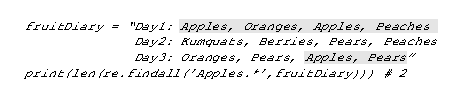
\includegraphics[width=\columnwidth]{../illustrations/lineSearch.eps}
}
\caption{An Example of Using .* to Count Lines Containing `Apples'}
\label{fig:lineSearch}
\end{figure}

In many cases, this \verb!`.*'! at the end of the string may not actually contribute any new behavior to the pattern, and may in fact be extraneous.  Or users may be trying to bypass the whole-string nature of the {\tt re.match} function, without realizing that they could instead use the {\tt re.search} function.  Consider the comparison shown in Figure~\ref{fig:searchVSmatch}

\begin{figure}[tb]
\centering
\fbox{
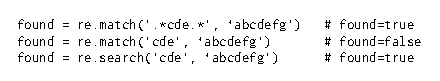
\includegraphics[width=\columnwidth]{../illustrations/matchVSsearch.eps}
}
\caption{An Example of Using .* to get Search Behavior From The Match Function}
\label{fig:searchVSmatch}
\end{figure}

Are programmers using the dot-star sub-pattern unnecessarily? More research is needed into this question to find out if these patterns are a candidate for refactoring.



% to find the largest count for the 'utilizing files' row: select distinct uniqueSourceID, filePath, count(distinct filePath) as ct from RegexCitationMerged group by uniqueSourceID order by ct;


% \subsubsection{default character classes are widely used}

%  Specifically, \verb!\s!, \verb!\d! and \verb!\W! were the top three behavioral clusters (as shown in Table~\ref{table:topNClusters}).  In Table~\ref{table:threeClusterSample} we show the top 10 patterns from these top three clusters. \todo{implication for tool designers}

% 
\begin{table}
\begin{center}
\caption{Top 10 Patterns in Top 3 Clusters (RQ3)}
\label{table:threeClusterSample}

\begin{tabular}
{c|c|c}
\toprule
example & example & example\\
\midrule
\begin{minipage}{0.5in}\begin{verbatim}`\s'\end{verbatim}\end{minipage} & \begin{minipage}{0.5in}\begin{verbatim}`\s'\end{verbatim}\end{minipage} & \begin{minipage}{0.5in}\begin{verbatim}`\s'\end{verbatim}\end{minipage}\\
\midrule
\begin{minipage}{0.5in}\begin{verbatim}`\s'\end{verbatim}\end{minipage} & \begin{minipage}{0.5in}\begin{verbatim}`\s'\end{verbatim}\end{minipage} & \begin{minipage}{0.5in}\begin{verbatim}`\s'\end{verbatim}\end{minipage}\\
\midrule
\begin{minipage}{0.5in}\begin{verbatim}`\s'\end{verbatim}\end{minipage} & \begin{minipage}{0.5in}\begin{verbatim}`\s'\end{verbatim}\end{minipage} & \begin{minipage}{0.5in}\begin{verbatim}`\s'\end{verbatim}\end{minipage}\\
\midrule
\begin{minipage}{0.5in}\begin{verbatim}`\s'\end{verbatim}\end{minipage} & \begin{minipage}{0.5in}\begin{verbatim}`\s'\end{verbatim}\end{minipage} & \begin{minipage}{0.5in}\begin{verbatim}`\s'\end{verbatim}\end{minipage}\\
\midrule
\begin{minipage}{0.5in}\begin{verbatim}`\s'\end{verbatim}\end{minipage} & \begin{minipage}{0.5in}\begin{verbatim}`\s'\end{verbatim}\end{minipage} & \begin{minipage}{0.5in}\begin{verbatim}`\s'\end{verbatim}\end{minipage}\\
\midrule
\begin{minipage}{0.5in}\begin{verbatim}`\s'\end{verbatim}\end{minipage} & \begin{minipage}{0.5in}\begin{verbatim}`\s'\end{verbatim}\end{minipage} & \begin{minipage}{0.5in}\begin{verbatim}`\s'\end{verbatim}\end{minipage}\\
\midrule
\begin{minipage}{0.5in}\begin{verbatim}`\s'\end{verbatim}\end{minipage} & \begin{minipage}{0.5in}\begin{verbatim}`\s'\end{verbatim}\end{minipage} & \begin{minipage}{0.5in}\begin{verbatim}`\s'\end{verbatim}\end{minipage}\\
\midrule
\begin{minipage}{0.5in}\begin{verbatim}`\s'\end{verbatim}\end{minipage} & \begin{minipage}{0.5in}\begin{verbatim}`\s'\end{verbatim}\end{minipage} & \begin{minipage}{0.5in}\begin{verbatim}`\s'\end{verbatim}\end{minipage}\\
\midrule
\begin{minipage}{0.5in}\begin{verbatim}`\s'\end{verbatim}\end{minipage} & \begin{minipage}{0.5in}\begin{verbatim}`\s'\end{verbatim}\end{minipage} & \begin{minipage}{0.5in}\begin{verbatim}`\s'\end{verbatim}\end{minipage}\\
\midrule
\begin{minipage}{0.5in}\begin{verbatim}`\s'\end{verbatim}\end{minipage} & \begin{minipage}{0.5in}\begin{verbatim}`\s'\end{verbatim}\end{minipage} & \begin{minipage}{0.5in}\begin{verbatim}`\s'\end{verbatim}\end{minipage}\\
\bottomrule
\end{tabular}
\end{center}
\end{table}



% example with anchors and {\tt .*} in the middle which could be replaced by a comma?














% Fun fact: while creating similarity matrix, row 5464 took 2 hours, or almost 1 second per cell avg, only suffering 18 timeouts (1.2 secs).  What is this pesky pattern?

% We do not assume that Python projects represent a perfect sample of regular expression usage in all environments, but to make the work of collecting data for the paper reasonable, we had to choose one language to focus on (we hope to compare results across languages in future work).  Python is an attractive choice because the culture of Python programming makes it seem likely that someone would write the pattern directly in the function, not trying to over-complicate things with some extra Classes or functions.  Other attractive choices are Perl (which probably has the most active regex community), javascript and ruby (which may emphasize web tasks like form validation), sql or a general purpose language like java or C\#.



